\section{Appendix}
\label{sec:Appendix}

\subsection{List of bird species}
\label{sec:Appendix1}

\begin{longtable}{clll}
    \caption{List of bird species used in this project. The classification label, the scientific name, as well as the english and german names of the species are listed.} 
    \label{tab:species} \\
    \toprule
    \textbf{Label} & \textbf{Scientific Name} & \textbf{English Name} & \textbf{German Name} \\
    \midrule
    \endfirsthead
    
    \toprule
    \textbf{Label} & \textbf{Scientific Name} & \textbf{English Name} & \textbf{German Name} \\
    \midrule
    \endhead
    
    \midrule
    \multicolumn{4}{r}{\textit{Continued on next page}} \\
    \midrule
    \endfoot
    
    \bottomrule
    \endlastfoot
    \small
    0 & \textit{Hirundo rustica} & Barn Swallow & Rauchschwalbe \\
    1 & \textit{Phoenicurus ochruros} & Black Redstart & Hausrotschwanz \\
    2 & \textit{Turdus merula} & Common Blackbird & Amsel \\
    3 & \textit{Fringilla coelebs} & Common Chaffinch & Buchfink \\
    4 & \textit{Phylloscopus collybita} & Common Chiffchaff & Zilpzalp \\
    5 & \textit{Cuculus canorus} & Common Cuckoo & Kuckuck \\
    6 & \textit{Luscinia megarhynchos} & Common Nightingale & Nachtigall \\
    7 & \textit{Tringa totanus} & Common Redshank & Rotschenkel \\
    8 & \textit{Phoenicurus phoenicurus} & Common Redstart & Gartenrotschwanz \\
    9 & \textit{Gallinago gallinago} & Common Snipe & Bekassine \\
    10 & \textit{Sturnus vulgaris} & Common Starling & Star \\
    11 & \textit{Columba palumbus} & Common Wood Pigeon & Ringeltaube \\
    12 & \textit{Prunella modularis} & Dunnock & Heckenbraunelle \\
    13 & \textit{Botaurus stellaris} & Eurasian Bittern & Rohrdommel \\
    14 & \textit{Sylvia atricapilla} & Eurasian Blackcap & Mönchsgrasmücke \\
    15 & \textit{Cyanistes caeruleus} & Eurasian Blue Tit & Blaumeise \\
    16 & \textit{Pyrrhula pyrrhula} & Eurasian Bullfinch & Gimpel \\
    17 & \textit{Streptopelia decaocto} & Eurasian Collared Dove & Türkentaube \\
    18 & \textit{Numenius arquata} & Eurasian Curlew & Großer Brachvogel \\
    19 & \textit{Bubo bubo} & Eurasian Eagle-Owl & Uhu \\
    20 & \textit{Oriolus oriolus} & Eurasian Golden Oriole & Pirol \\
    21 & \textit{Garrulus glandarius} & Eurasian Jay & Eichelhäher \\
    22 & \textit{Sitta europaea} & Eurasian Nuthatch & Kleiber \\
    23 & \textit{Spinus spinus} & Eurasian Siskin & Erlenzeisig \\
    24 & \textit{Passer montanus} & Eurasian Tree Sparrow & Feldsperling \\
    25 & \textit{Scolopax rusticola} & Eurasian Woodcock & Waldschnepfe \\
    26 & \textit{Troglodytes troglodytes} & Eurasian Wren & Zaunkönig \\
    27 & \textit{Lophophanes cristatus} & European Crested Tit & Haubenmeise \\
    28 & \textit{Carduelis carduelis} & European Goldfinch & Stieglitz \\
    29 & \textit{Chloris chloris} & European Greenfinch & Grünfink \\
    30 & \textit{Erithacus rubecula} & European Robin & Rotkehlchen \\
    31 & \textit{Regulus regulus} & Goldcrest & Wintergoldhähnchen \\
    32 & \textit{Parus major} & Great Tit & Kohlmeise \\
    33 & \textit{Passer domesticus} & House Sparrow & Haussperling \\
    34 & \textit{Athene noctua} & Little Owl & Steinkauz \\
    35 & \textit{Charadrius dubius} & Little Ringed Plover & Flussregenpfeifer \\
    36 & \textit{Asio otus} & Long-eared Owl & Waldohreule \\
    37 & \textit{Anthus pratensis} & Meadow Pipit & Wiesenpieper \\
    38 & \textit{Turdus viscivorus} & Mistle Thrush & Misteldrossel \\
    39 & \textit{Vanellus vanellus} & Northern Lapwing & Kiebitz \\
    40 & \textit{Turdus iliacus} & Redwing & Rotdrossel \\
    41 & \textit{Turdus philomelos} & Song Thrush & Singdrossel \\
    42 & \textit{Strix aluco} & Tawny Owl & Waldkauz \\
    43 & \textit{Motacilla alba} & White Wagtail & Bachstelze \\
    44 & \textit{Phylloscopus trochilus} & Willow Warbler & Fitis \\
    45 & \textit{Emberiza citrinella} & Yellowhammer & Goldammer \\
    \end{longtable}

\subsection{Class distributions for training and test data}
\label{sec:Appendix2}

\begin{figure}
    \centering
    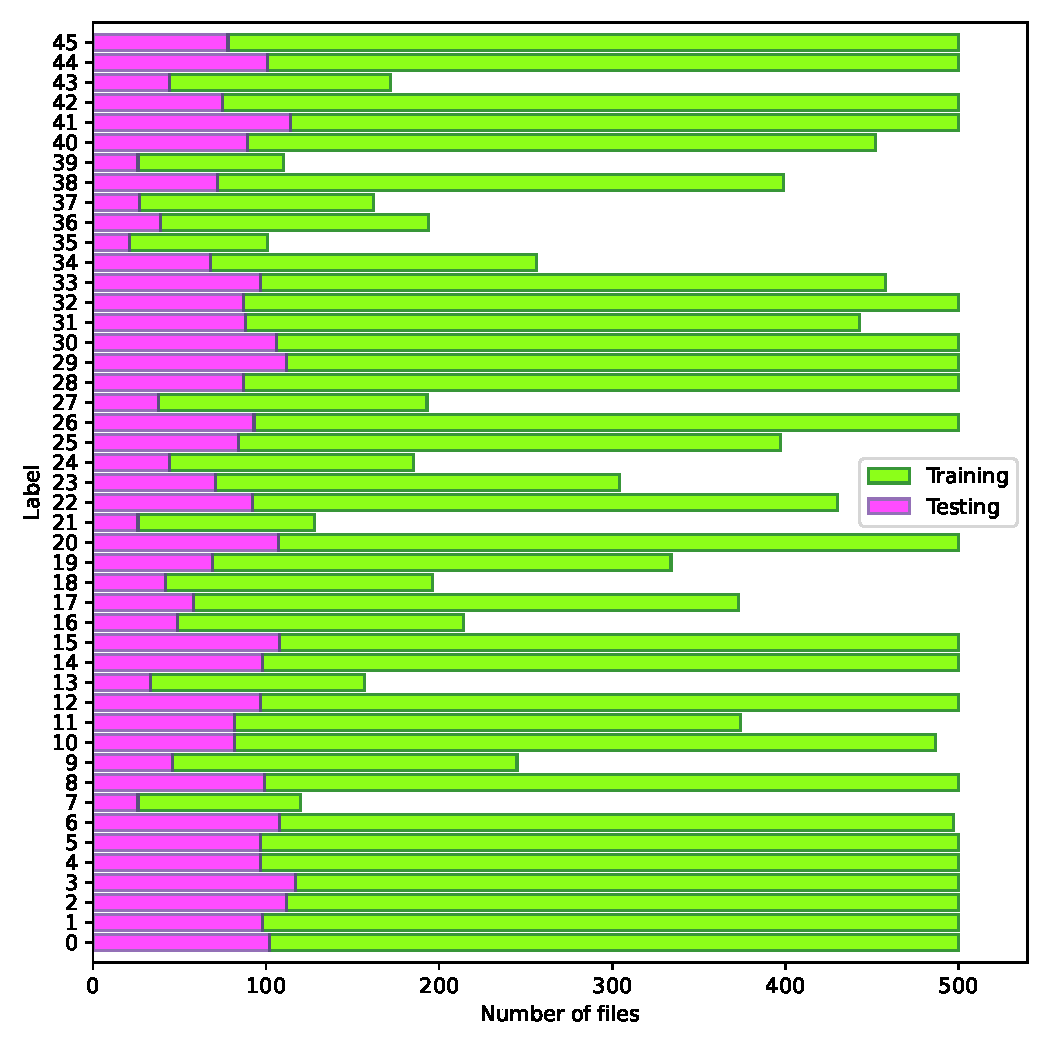
\includegraphics[width = .6\textwidth]{content/plots/class_distributions.pdf}
    \caption{Class distributions of the number of files for training and test dataset (stacked). As can be seen, the classes are imbalanced.}
    \label{fig:class_distributions}
\end{figure}

\begin{figure}
    \centering
    \includegraphics[width = .6\textwidth]{content/plots/class_distributions_length.pdf}
    \caption{Class distributions of the total audio length for training and test dataset (stacked). The imbalance gets more severe due to the fact, that classes with a lower 
    number of files tend to also have shorter recordings.}
    \label{fig:class_distributions_length}
\end{figure}

\subsection{Additional material on the hyperparameter optimization}
\label{sec:Appendix3}

\begin{figure}
    \centering 
    \includegraphics[width = .8\textwidth]{content/plots/sweep3.png}
    \caption{Hyperparamters of the third sweep and their impact on validation accuracy. A new activation function, the \enquote{mish} activation function is also tested but not found 
    to yield better results. The study on the dropout percentages is inconclusive.}
    \label{fig:sweep3}
\end{figure}

\newpage

\subsection{Audio features used for the $\mathbf{k}$NN classifier}
\label{sec:Appendix4}
\begin{table}[h]
    \centering
    \small
    \caption{List of Extracted Audio Features}
    \label{tab:features}
    \begin{tabular}{>{\raggedright\arraybackslash}p{0.3\textwidth} >{\raggedright\arraybackslash}p{0.6\textwidth}}
        \toprule
        \textbf{Feature} (count) & \textbf{Description} \\
        \midrule
        Zero Crossing Rate & The rate at which the signal changes sign. \\
        Root Mean Square Energy & The square root of the average of the squared values of the signal, representing signal power. \\
        Spectral Centroid & The "center of mass" of the spectrum, indicating where the bulk of the energy is concentrated. \\
        Spectral Bandwidth & The width of the spectrum, representing the spread of frequencies around the centroid. \\
        Spectral Flatness & A measure of how flat or peaky a spectrum is. High flatness indicates noise-like signals. \\
        Spectral Rolloff  & The frequency below which a certain percentage of the total spectral energy is contained. \\
        \midrule
        Mean & The average amplitude of the audio signal. \\
        Standard Deviation & The amount of variation or dispersion of the audio signal. \\
        Skewness & The asymmetry of the signal amplitude distribution. \\
        Kurtosis & The "tailedness" of the signal amplitude distribution. \\
        \midrule
        Mel-frequency Cepstral Coefficients (10) & A set of coefficients that represent the short-term power spectrum of the audio signal. \\
        Spectral Contrast (7) & The difference between peaks and valleys in the spectrum, calculated in sub-bands. \\
        Chroma Features (12) & The distribution of energy across the 12 pitch classes of the chromatic scale. \\
        Tonnetz (6) & Harmonic and tonal features representing the tonal centroid features of the signal. \\
        \bottomrule
    \end{tabular}
\end{table}
